%
%  f2h
%
%  Created by Martell on 2012-03-16.
%  Copyright (c) 2012 UBC Fisheries Centre. All rights reserved.
%
\documentclass{beamer}
%\usetheme{Madrid} % My favorite!
%\usetheme{PaloAlto}
\usetheme{Goettingen}
%\usetheme{Hannover}
%\usetheme{Boadilla} % Pretty neat, soft color.
%\usetheme{default}
%\usetheme{Warsaw}
%\usetheme{Bergen} % This template has nagivation on the left
%\usetheme{Frankfurt} % Similar to the default 
%with an extra region at the top.
%\usecolortheme{seahorse} % Simple and clean template
%\usecolortheme{beaver}
%\usetheme{Darmstadt} % not so good
% Uncomment the following line if you want %
% page numbers and using Warsaw theme%
% \setbeamertemplate{footline}[page number]
%\setbeamercovered{transparent}
\setbeamercovered{invisible}
% To remove the navigation symbols from 
% the bottom of slides%
\setbeamertemplate{navigation symbols}{} 
%
\usepackage{color}
\usepackage{graphicx}
\usepackage{apacite}
\usepackage{amssymb}
\usepackage{amsmath}
%\usepackage{bm}         % For typesetting bold math (not \mathbold)
%\logo{\includegraphics[height=0.6cm]{yourlogo.eps}}
%

\definecolor{bottomcolour}{rgb}{0.32,0.3,0.38}
\definecolor{middlecolour}{rgb}{0.08,0.08,0.16}
\setbeamerfont{title}{size=\Huge}
\setbeamercolor{structure}{fg=white}
\setbeamertemplate{frametitle}[default][center]

\setbeamercolor{normal text}{bg=black, fg=white}
\setbeamertemplate{background canvas}[vertical shading]
[bottom=bottomcolour, middle=middlecolour, top=black]

\setbeamertemplate{itemize item}{\lower3pt\hbox{\Large\textbullet}}
\setbeamerfont{frametitle}{size=\huge}


\title[Steepness]{Deriving Steepness from \fmsy\ or \fspr}
\author{Steven Martell}
\institute[UBC]
{
University of British Columbia \\
\medskip
{\emph{s.martell@mail.ubc.ca}}
}
\date{\today}
% \today will show current date. 
% Alternatively, you can specify a date.
%

\newcommand{\fmsy}{$\rm{F_{MSY}}$}
\newcommand{\fspr}{$\rm{F_{SPR}}$}

\begin{document}
%
\begin{frame}
\titlepage
\end{frame}
%
\section{Motivation} % (fold)
\label{sec:motivation}

\begin{frame}
\frametitle{Motivation}
\begin{block}
{Why do we use proxies for \fmsy?}
\end{block}
\begin{itemize}
	\item<+-> On rare occasions \fmsy\ is estimable.
	\begin{itemize}
		\item Stock-recruitment data required
	\end{itemize}
	\item<+-> \fspr\ requires only life-history information.
	\begin{itemize}
		\item Natural mortality rate, fecundity, growth, ...
		\item<+-> F$_{35\%}$ can achieve $\approx$ 80\% of MSY \cite{clark1991groundfish}.
		\item<+-> F$_{35\%}$ can lead to severe depletion \cite{clark2002f}.
	\end{itemize}
\end{itemize}
\end{frame}
% section motivation (end)
%
%
%
%
\section{Deriving \fmsy} % (fold)
\label{sec:deriving_fmsy}
\begin{frame}
\frametitle{Deriving \fmsy}
\only<1>{
\begin{block}{$(B_0,h)\Rightarrow$ (MSY,\fmsy) transition}
	
	Estimated parameters used to derived reference points
	\begin{columns}
		\begin{column}{0.5\textwidth}
			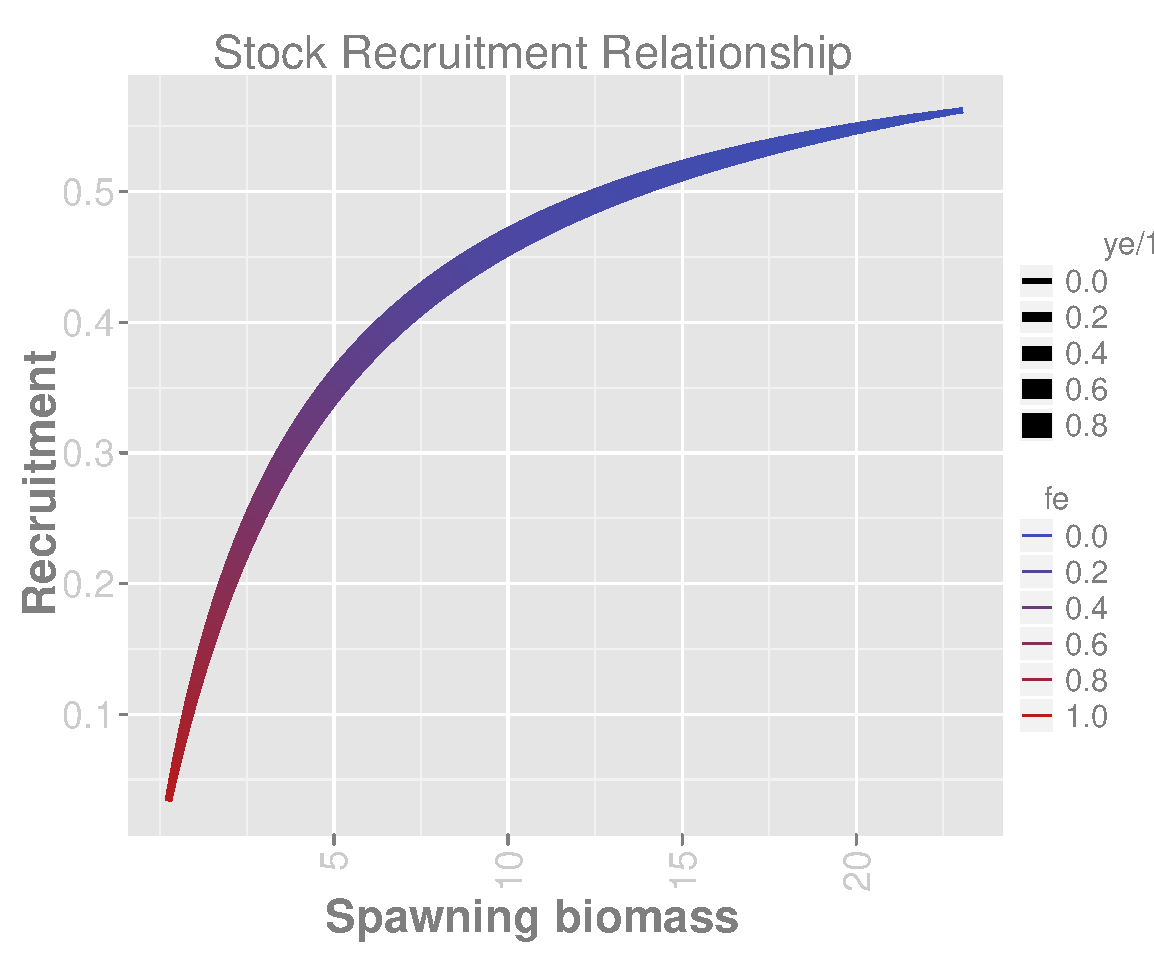
\includegraphics[height=0.8\textwidth]{../figStockRecruitII.pdf}
		\end{column}
		\begin{column}{0.5\textwidth}
			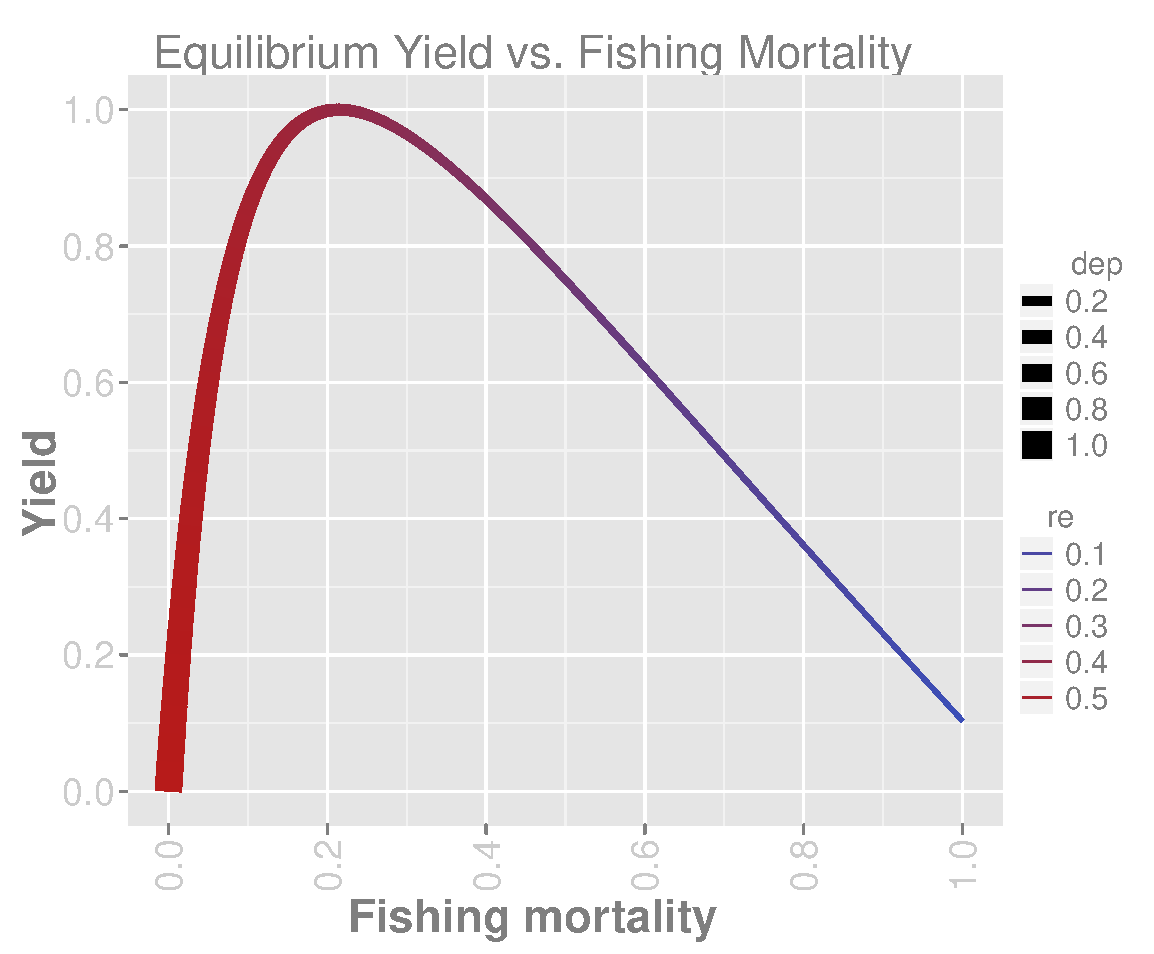
\includegraphics[height=0.8\textwidth]{../figEquilYield.pdf}
		\end{column}
	\end{columns}
\end{block}
}
\only<2>{
Given $\Theta=(B_0,h,M,f_a,s_a)$,\\ \fmsy\ is calculated by maximizing:
\begin{align}
	C_e &= F_e g(\Theta) \\
	\frac{\partial C_e}{\partial F_e}&= 
	g(\Theta) + F_e g(\Theta) \frac{\partial g(\Theta)}{\partial F_e}\label{eq2} 
\end{align}
Set (2) equal to 0 and \underline{numerically} solve for $F_e$.
}
\end{frame}
% section deriving_fmsy (end)
%
%
%
%
\section{Deriving h} % (fold)
\label{sec:deriving_h}
\begin{frame}[fragile]\frametitle{Deriving steepness ($h$) from \fmsy}
\only<1>{
\begin{block}{(MSY,\fmsy) $\Rightarrow(B_0,h)$ transition}
	In this case estimate reference points directly.
	\begin{columns}
		\begin{column}{0.49\textwidth}
			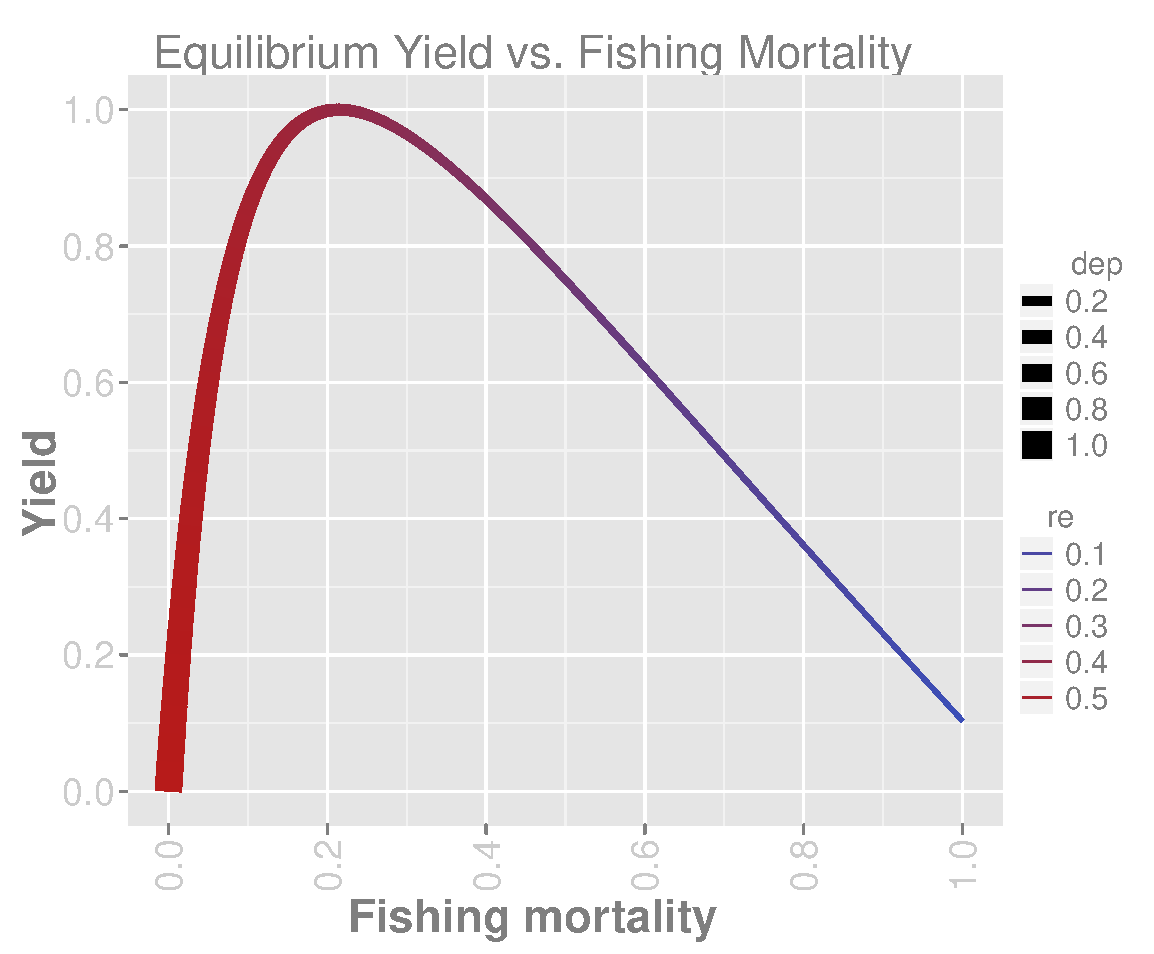
\includegraphics[height=0.8\textwidth]{../figEquilYield.pdf}
		\end{column}
		\begin{column}{0.49\textwidth}
			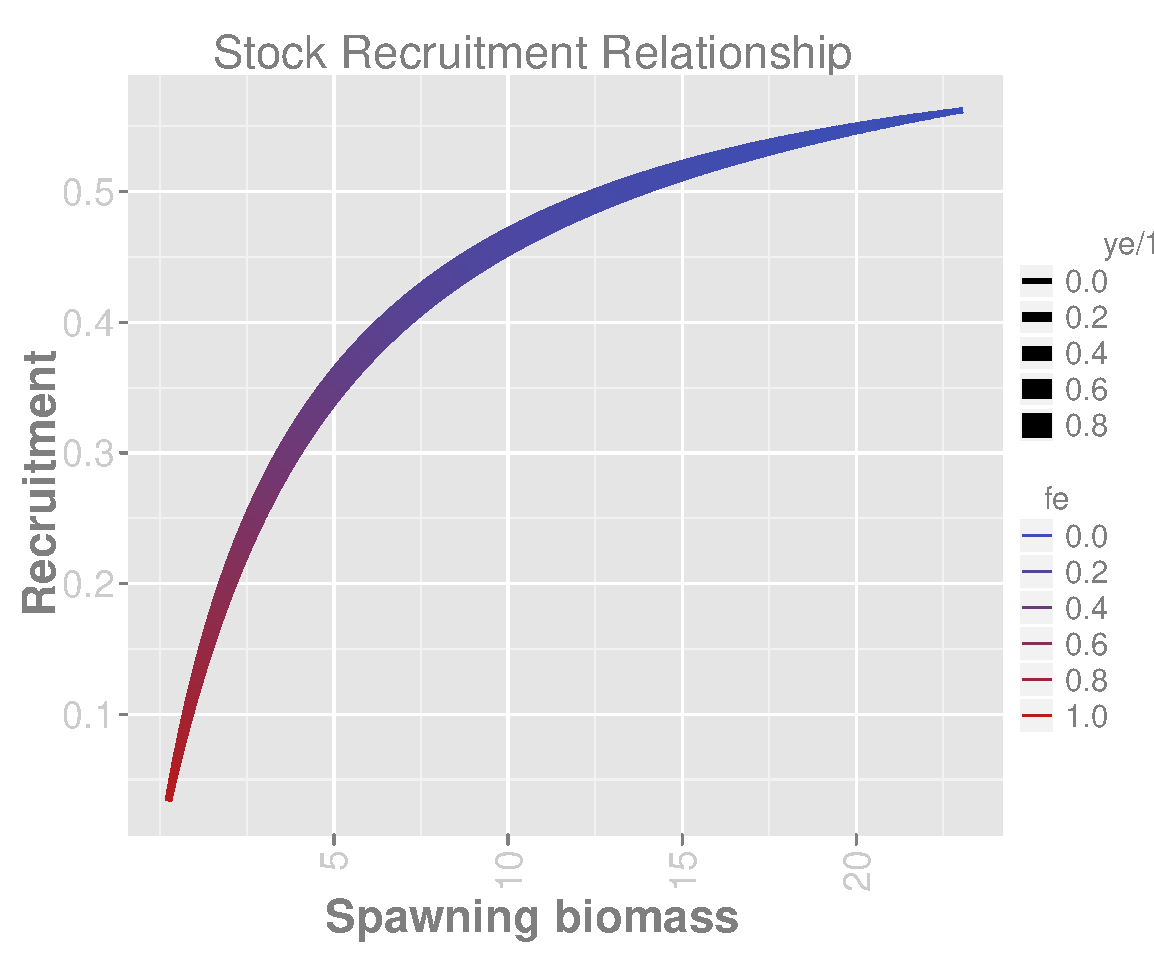
\includegraphics[height=0.8\textwidth]{../figStockRecruitII.pdf}
		\end{column}
	\end{columns}
\end{block}
}
\only<+->{
Given $\Theta=(\mathrm{MSY},\rm{F_{MSY}},M,f_a,s_a)$,\\ then solve the catch equation for $h$.
\pause

\begin{align}
	C_e &= F_e g(\Theta)   \\
	    &= F_e R_e \phi_q \\
	&\mbox{$R_e$ is the equilibrium recruitment (includes $h$)}\nonumber \\
	&\mbox{$\phi_q$ is the yield per recruit} \nonumber 
\end{align}
\pause
\begin{align}
	\frac{\partial C_e}{\partial F_e}&= 0=
	R_e \phi_q + F_e \phi_q \frac{\partial R_e}{\partial F_e} + F_e R_e \frac{\partial \phi_q}{\partial F_e}
	%g(\Theta) + F_e g(\Theta) \frac{\partial g(\Theta)}{\partial F_e}\label{eq4} 
\end{align}
In this case there is an Analytical solution for $h$ for Beverton-Holt \& Ricker models.
}
\end{frame}
% section deriving_h (end)
%
%
%
%
\section{Example} % (fold)
\label{sec:example}
\begin{frame}[t]\frametitle{Exampe: Pacific halibut}
	IPHC: fixed harvest rate of 21.5\%, what is the implied $h$?
	\pause
	\only<2>{
	\begin{figure}[htbp]
		\centering
			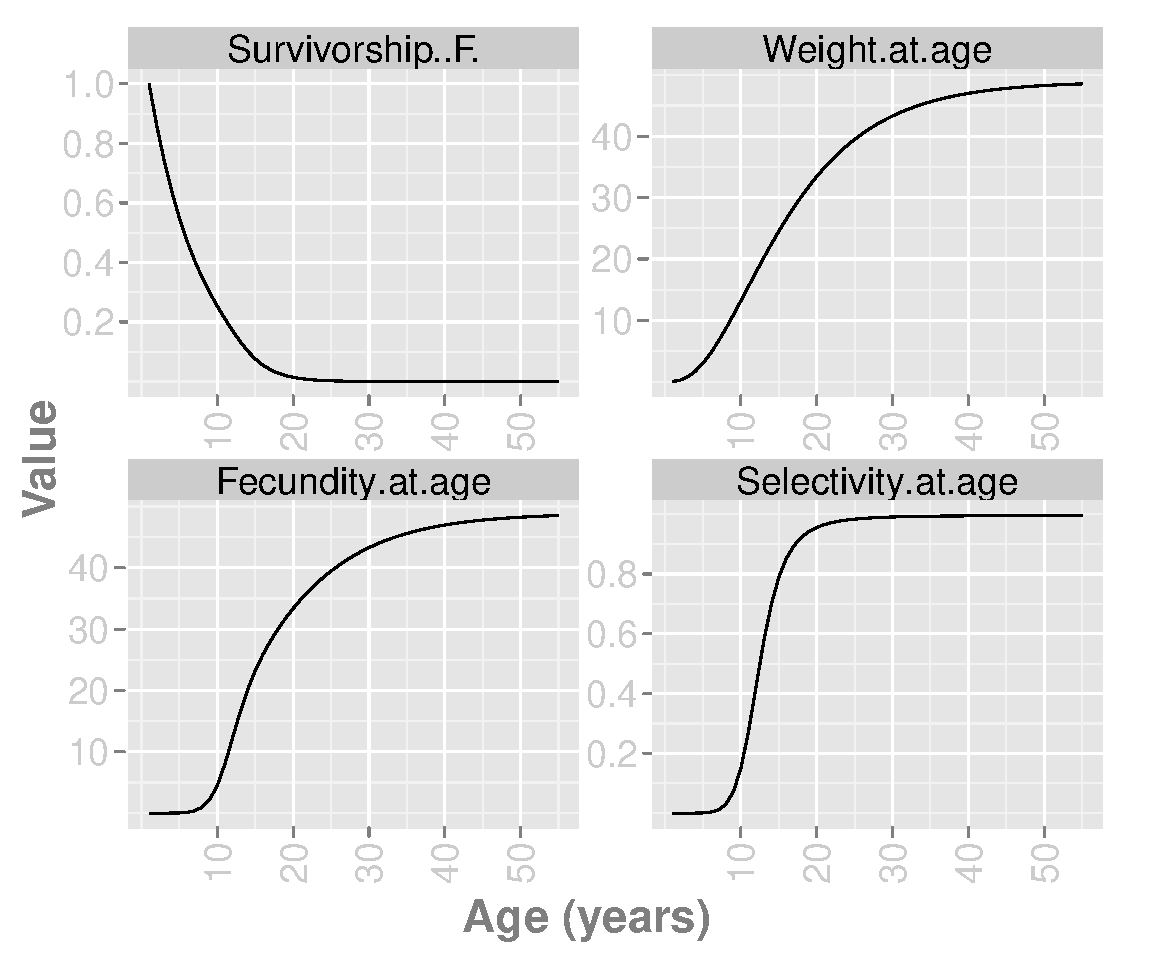
\includegraphics[height=2.4in]{../figHalibutAgeSchedules.pdf}
		\caption{Pacific halibut life-history \& selectivity.}
		\label{fig:figHalibutAgeSchedules}
	\end{figure}
	}
	\only<3>{
	\begin{figure}[htbp]
		\centering
			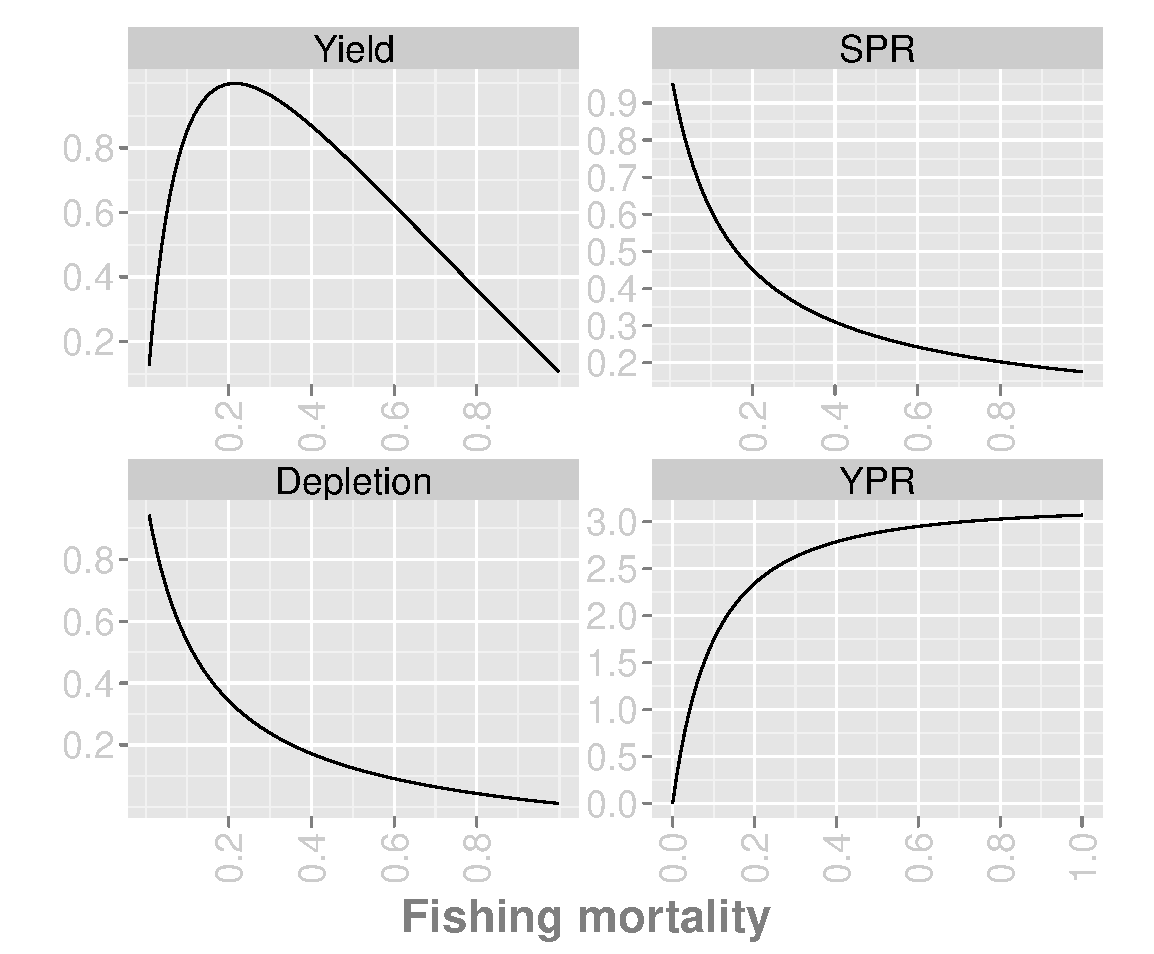
\includegraphics[height=2.4in]{../figHalibutEquilYield.pdf}
		\caption{Yield, depletion, SPR and YPR for Pacific halibut.}
		\label{fig:figHalibutEquilYield}
	\end{figure}
	}
	\only<4>{
	\begin{figure}[htbp]
		\centering
			\includegraphics[height=2.4in]{../figStockRecruitSteepness.pdf}
		\caption{Steepness ($h=0.5997$) for the assumed \fmsy=0.215.}
		\label{fig:figStockRecruitSteepness}
	\end{figure}
	
	}
\end{frame}
%
\begin{frame}[t]\frametitle{Relationship between \fmsy\ and $h$}
	\only<1>{
	\begin{figure}[htbp]
		\centering
			\includegraphics[height=2.4in]{../figFMSYSteepness.pdf}
		\caption{Exponential increase in \fmsy with increasing $h$}
		\label{fig:figFMSYSteepness}
	\end{figure}
	}
	\only<2>{
	\begin{figure}[htbp]
		\centering
			\includegraphics[height=2.4in]{../figSteepVsOther.pdf}
		\caption{Relationship between $h$ and other population parameters.}
		\label{fig:figSteepVsOther}
	\end{figure}
	
	}
\end{frame}
%
\begin{frame}[t]\frametitle{Deriving implied priors for steepness}
	\only<1>{
	\begin{figure}[htbp]
		\centering
			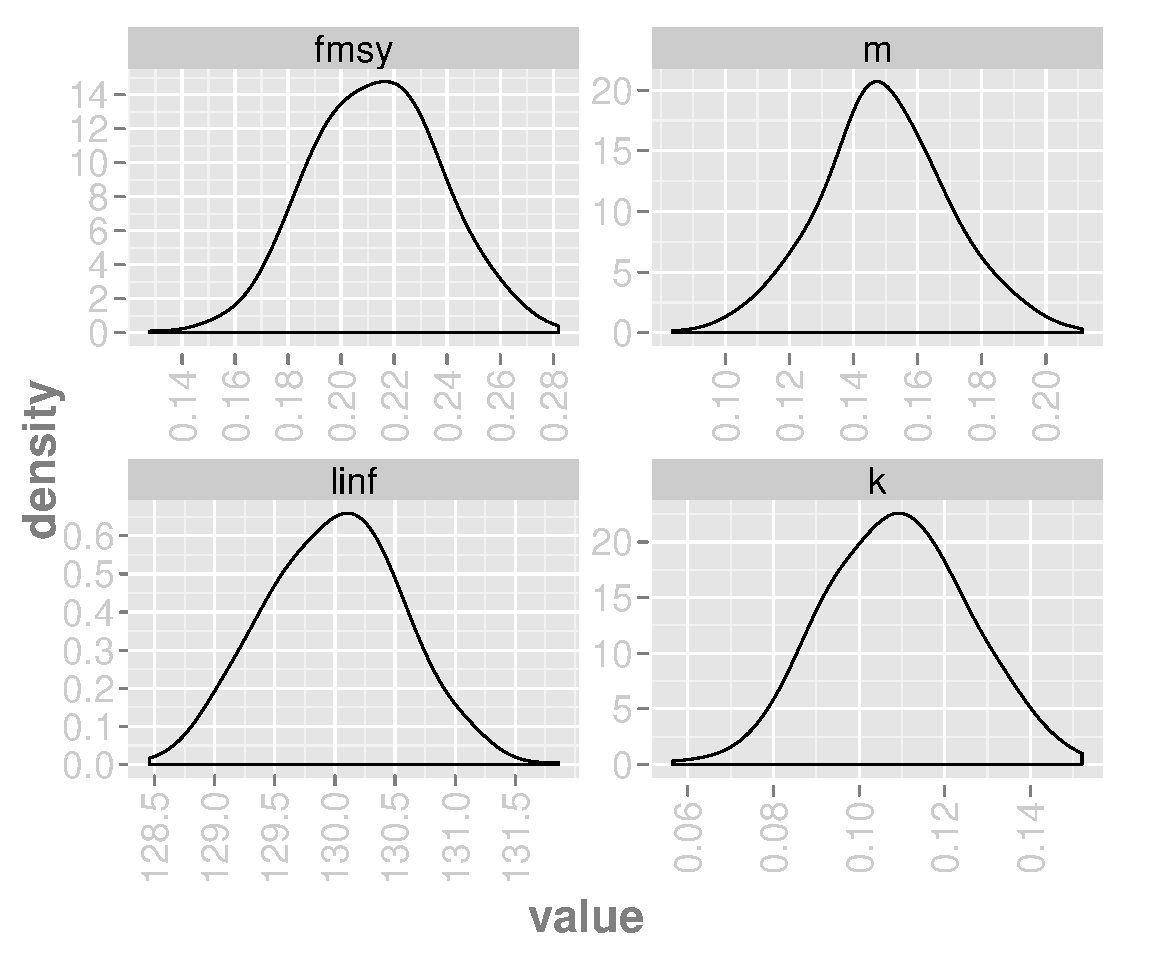
\includegraphics[height=2.4in]{../figThetaPrior.pdf}
		\caption{Prior densities for \fmsy, natural mortality, growth, imply ...}
		\label{fig:figThetaPrior}
	\end{figure}
	}
	\only<2>{
	\begin{figure}[htbp]
		\centering
			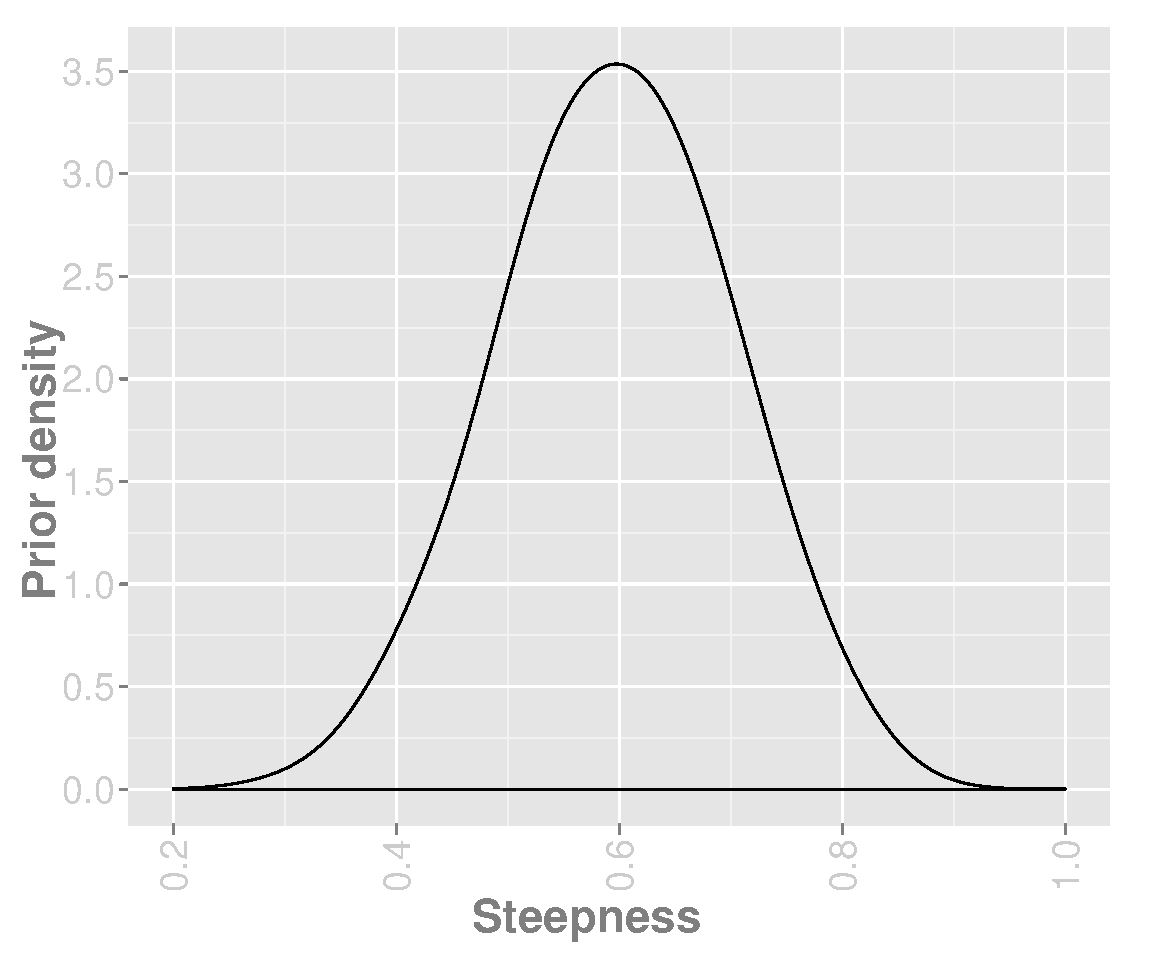
\includegraphics[height=2.4in]{../figSteepnessPrior.pdf}
		\caption{Prior density for steepness.}
		\label{fig:figSteepnessPrior}
	\end{figure}
	
	}
\end{frame}
% section example (end)
%
%
\section{Summary} % (fold)
\label{sec:summary}
\begin{frame}[t]\frametitle{Summary}
	\begin{itemize}
		\item<+->  \fmsy\ proxy implies steepness is known.
		\begin{itemize}
			\item Use \fmsy $\Rightarrow h$ transition in assessment models for consistency.
			\item Alternative: fix $h$, which may be inconsistent with proxy.
		\end{itemize}
		\item<+-> Steepness is confounded with other key population parameters/reference points.
		\item<+-> Choice of \fmsy\ proxy implies prior density for $h$.
		\item<+-> Parametrize with (\fmsy, MSY) instead of ($B_0, h$) \cite{Martell2008pam}.
		\item<+-> Not to be used with Hierarchical models for generating Posterior predictive distributions.
		\begin{itemize}
			\item Definition of a recruit is a vulnerable fish of any age.
		\end{itemize}
	\end{itemize}
\end{frame}
% section summary (end)
%
%

\begin{frame}\frametitle{References}
\scriptsize{
\bibliographystyle{apacite}
\bibliography{$HOME/Documents/ARTICLES/Articles-1}
}
Rcode for .fmsy2h available from me.
\end{frame}
 
\begin{frame}
	\frametitle{Acknowledgements}
	IPHC for office space.
	\vfill
	Swedish Medical Center for pain relief.
	

\end{frame}
% End of slides


\end{document}

